\documentclass[a4paper,landscape,9pt]{article}

\usepackage[margin=1cm]{geometry}
\usepackage{fontspec}
\setmainfont{TeX Gyre Pagella}
\usepackage{unicode-math}
\setmathfont{TeX Gyre Pagella Math}

\usepackage{tikz}
\usetikzlibrary{arrows.meta,calc,positioning,shapes.geometric}
\usepackage{microtype}

\pagestyle{empty}
\setlength{\parindent}{0pt}
\setlength{\parskip}{0.25em}

\tikzset{
  node-d/.style={draw,fill=black,regular polygon,regular polygon sides=6,minimum size=7mm,inner sep=0pt,text=white,font=\tiny\bfseries},
  node-a/.style={draw,fill=black!70,regular polygon,regular polygon sides=3,minimum size=7mm,inner sep=0pt,text=white,font=\tiny\bfseries},
  node-t/.style={draw,circle,minimum size=7mm,inner sep=0pt,line width=0.4pt,font=\tiny},
  node-o/.style={draw,fill=black!15,rectangle,minimum size=7mm,inner sep=0pt,font=\tiny},
  node-i/.style={draw,diamond,minimum size=8mm,inner sep=0pt,line width=0.4pt,font=\tiny},
  impl/.style={-{Latex[length=1.2mm]},line width=0.3pt,black!80},
  exemp/.style={-{Latex[length=1.2mm]},line width=0.3pt,dashed,black!80},
  band/.style={font=\scriptsize\scshape,text=black!60},
  bandline/.style={draw,black!18,line width=0.3pt},
}

\begin{document}

\begin{center}
{\large\scshape Proposisjonsgraf, seksjon 4}\hspace{0.8em}{\itshape Landskapet er dynamisk}
\end{center}

\vspace{-0.6em}

\begin{center}
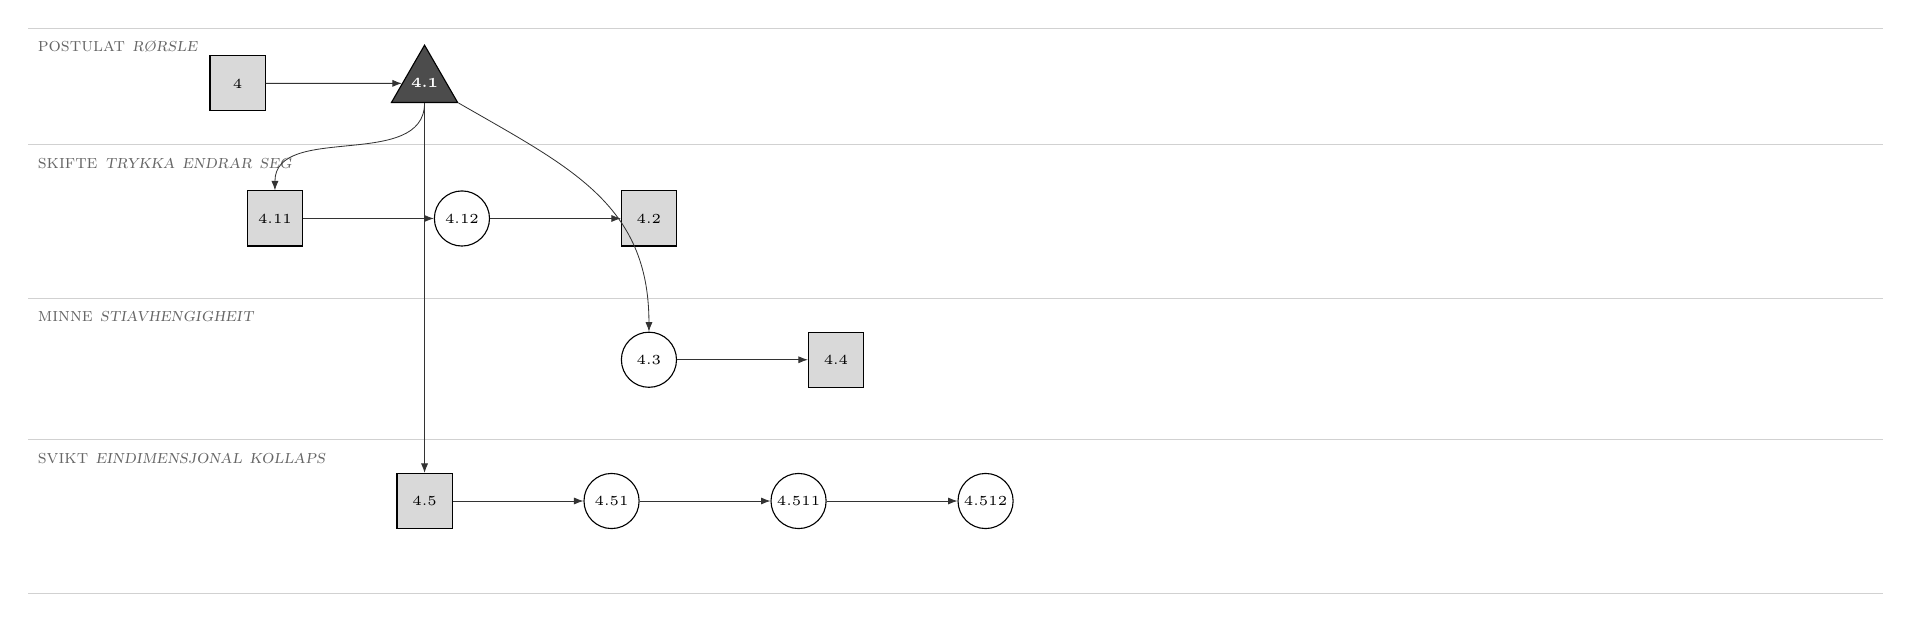
\begin{tikzpicture}[x=0.95cm,y=0.78cm]

  \draw[bandline] (-0.3, 0.6)   -- (24.5, 0.6);
  \draw[bandline] (-0.3, -1.3)  -- (24.5, -1.3);
  \draw[bandline] (-0.3, -3.8)  -- (24.5, -3.8);
  \draw[bandline] (-0.3, -6.1)  -- (24.5, -6.1);
  \draw[bandline] (-0.3, -8.6)  -- (24.5, -8.6);

  \node[band,anchor=west] at (-0.3, 0.3)  {postulat  \itshape rørsle};
  \node[band,anchor=west] at (-0.3, -1.6) {skifte  \itshape trykka endrar seg};
  \node[band,anchor=west] at (-0.3, -4.1) {minne  \itshape stiavhengigheit};
  \node[band,anchor=west] at (-0.3, -6.4) {svikt  \itshape eindimensjonal kollaps};

  % BAND 1: postulat
  \node[node-o] (p4)      at (2.5, -0.3)  {4};
  \node[node-a] (p41)     at (5, -0.3)    {4.1};
  \draw[impl] (p4) -- (p41);

  % BAND 2: skifte
  \node[node-o] (p411)    at (3, -2.5)    {4.11};
  \node[node-t] (p412)    at (5.5, -2.5)  {4.12};
  \node[node-o] (p42)     at (8, -2.5)    {4.2};
  \draw[impl] (p41)  to[out=-90,in=90] (p411);
  \draw[impl] (p411) -- (p412);
  \draw[impl] (p412) -- (p42);

  % BAND 3: minne
  \node[node-t] (p43)     at (8, -4.8)    {4.3};
  \node[node-o] (p44)     at (10.5, -4.8) {4.4};
  \draw[impl] (p41) to[out=-30,in=90,looseness=1.1] (p43);
  \draw[impl] (p43) -- (p44);

  % BAND 4: svikt
  \node[node-o] (p45)     at (5, -7.1)    {4.5};
  \node[node-t] (p451)    at (7.5, -7.1)  {4.51};
  \node[node-t] (p4511)   at (10, -7.1)   {4.511};
  \node[node-t] (p4512)   at (12.5, -7.1) {4.512};
  \draw[impl] (p41)  to[out=-90,in=90,looseness=0.9] (p45);
  \draw[impl] (p45)  -- (p451);
  \draw[impl] (p451) -- (p4511);
  \draw[impl] (p4511) -- (p4512);

\end{tikzpicture}
\end{center}

\vspace{-0.2em}

\hrule

\vspace{0.4em}

\begin{minipage}[t]{0.325\textwidth}
{\scshape\small Lesing ovanfrå}

Rota \emph{4} er observasjonen at landskapet er dynamisk. Band 1 gjer han presis gjennom eit einsamt postulat: \emph{4.1} seier at \textbf{seleksjonstrykka kviler aldri}. Dette er seksjonens einaste triangel, og han ber heile vekta av det som følgjer.

Frå \emph{4.1} går det tre uavhengige kaskadar nedover gjennom seksjonens tre resterande band. Postulatet er dermed \emph{knutepunktet} som heile seksjonen heng i.
\end{minipage}\hfill
\begin{minipage}[t]{0.325\textwidth}
{\scshape\small Lesing nedover}

Band 2 karakteriserer \textbf{skifte}. \emph{4.11} namngjev drivkreftene: ny teknologi, marknad, materiale. \emph{4.12} seier at små endringar akkumulerer seg til topologisk kollaps. \emph{4.2} observerer mønsteret: lange stase-periodar brotne av brå skifte.

Band 3 karakteriserer \textbf{minne}. \emph{4.3} slår fast at landskapet hugsar; all formgjeving er omformgjeving. \emph{4.4} trekk konsekvensen: formrommet ekspanderer kumulativt.

Band 4 er seksjonens lengste kaskade: fire nodar i rekkje som dokumenterer \textbf{eindimensjonal kollaps}. Frå observasjonen at eitt trykk dominerer (\emph{4.5}), via det teoretiske namnet for fenomenet (systematisk blindskap, \emph{4.51}), til dei to konsekvensane: sviktande former (\emph{4.511}) og ureparabel fortrengt kompetanse (\emph{4.512}).
\end{minipage}\hfill
\begin{minipage}[t]{0.325\textwidth}
{\scshape\small Strukturelle innsikter}

\emph{Postulatsparsemd.} Eitt einaste triangel i heile seksjonen, og det ber alt. Formell stramheit på sitt reinaste.

\emph{Observasjonsovervekt.} Fem fylte kvadrat, fem sirklar (teorem), eitt einaste triangel. Seksjonen er empirisk tung; han dokumenterer kva dynamikk \emph{ser ut som}, ikkje kva ho logisk må vere.

\emph{Tre parallelle kaskadar.} Frå \emph{4.1} fanar det ut til tre uavhengige utviklingsliner, ein i kvart av band 2 til 4. Tidlegare seksjonar hadde færre greiner; denne har full treklang.

\emph{Ingen konfluens.} Hypotesa om karakteriseringsseksjonar held. Trass i postulatet, er seksjon 4 ein karakterisering av noko som allereie er innført.

\emph{Svikt-kaskaden.} Den lengste lineære kjeda i seksjonen (\emph{4.5} til \emph{4.512}) er nettopp der funksjonalisme-kritikken tek strukturelt plass. Kritikken er ikkje eit tillegg; han er innvevd.
\end{minipage}

\end{document}
